\section{Auswertung}
\label{sec:Auswertung}
\subsection{2V-Messung}
Die Messung von -2V bis 2V sollte für die rote, grüne und violette Spektrallinie mit der größten Intensität
aufgenommen werden. Dabei entspricht die rote Spektrallinie der Wellenlänge 623nm , die grüne der Wellenlänge 546nm und
die violette der Wellenlänge 435nm \cite{sample},\cite{Spektrum}.
\begin{table}[H]
  \centering
  \caption{Messwerte für die rote, grüne und violette Spektrallinie(1).}
  \label{tab:2VMesswerte(1)}
  \begin{tabular}{S[table-format=1.2] S[table-format=3] S[table-format=1.2] S[table-format=4]S[table-format=1.2]S[table-format=2]}
      \toprule
      {$U_\text{Grün}$/V}&{$I_\text{GrPh}$/pA}&{$U_\text{violett}$/V}&{$I_\text{ViPh}$/pA}&{$U_\text{Rot}$/V}&{$I_\text{RotPh}$/pA}\\
      \midrule
      -2 & -20 & -2 & -25 & -2 & 0 \\
      -1,9 & -20 & -1,9 & -24 & -1,9 & 0 \\
      -1,8 & -20 & -1,8 & -24 & -1,8 & 0 \\
      -1,7 & -20 & -1,7 & -24 & -1,7 & 0 \\
      -1,6 & -19 & -1,6 & -23 & -1,6 & 0 \\
      -1,5 & -19 & -1,5 & -22 & -1,5 & 0 \\
      -1,4 & -19 & -1,4 & -20 & -1,4 & 0 \\
      -1,3 & -19 & -1,3 & -18 & -1,3 & 0 \\
      -1,2 & -18 & -1,25 & -16 & -1,2 & 0 \\
      -1,1 & -17 & -1,2 & -13 & -1,1 & 0 \\
      -1 & -16 & -1,15 & -10 & -1 & 0 \\
      -0,9 & -16 & -1,1 & -6 & -0,9 & 0 \\
      -0,8 & -14 & -1,05 & -2 & -0,8 & 0 \\
      -0,7 & -10 & -1 & 1 & -0,7 & 0 \\
      -0,65 & -6 & -0,95 & 9 & -0,6 & 0 \\
      -0,6 & -1 & -0,9 & 18 & -0,5 & 1 \\
      -0,55 & 2 & -0,85 & 28 & -0,45 & 2 \\
      -0,5 & 15 & -0,8 & 41 & -0,4 & 2 \\
      -0,45 & 29 & -0,75 & 57 & -0,35 & 3 \\
      -0,4 & 49 & -0,7 & 74 & -0,3 & 4 \\
      -0,35 & 78 & -0,65 & 95 & -0,25 & 5 \\
      -0,3 & 110 & -0,6 & 110 & -0,2 & 6 \\
      -0,25 & 140 & -0,55 & 140 & -0,15 & 7 \\
      -0,2 & 160 & -0,5 & 150 & -0,1 & 8 \\
      -0,15 & 190 & -0,45 & 190 & -0,05 & 10 \\
      \bottomrule
  \end{tabular}
\end{table}

\begin{table}[H]
  \centering
  \caption{Messwerte für die rote, grüne und violette Spektrallinie(2).}
  \label{tab:2VMesswerte(2)}
  \begin{tabular}{S[table-format=1.2] S[table-format=3] S[table-format=1.2] S[table-format=4]S[table-format=1.2]S[table-format=2]}
      \toprule
      {$U_\text{Grün}$/V}&{$I_\text{GrPh}$/pA}&{$U_\text{violett}$/V}&{$I_\text{ViPh}$/pA}&{$U_\text{Rot}$/V}&{$I_\text{RotPh}$/pA}\\
      \midrule
      -0,1 & 220 & -0,4 & 210 & 0 & 11 \\
      -0,05 & 250 & -0,3 & 250 & 0,05 & 12 \\
      0 & 270 & -0,2 & 300 & 0,1 & 14 \\
      0,05 & 290 & -0,1 & 340 & 0,15 & 15 \\
      0,1 & 310 & 0 & 380 & 0,2 & 16 \\
      0,15 & 330 & 0,1 & 420 & 0,25 & 18 \\
      0,2 & 350 & 0,2 & 460 & 0,3 & 19 \\
      0,3 & 390 & 0,3 & 490 & 0,35 & 20 \\
      0,4 & 420 & 0,4 & 530 & 0,4 & 22 \\
      0,5 & 460 & 0,5 & 560 & 0,5 & 24 \\
      0,6 & 480 & 0,6 & 600 & 0,6 & 26 \\
      0,7 & 520 & 0,7 & 630 & 0,7 & 29 \\
      0,8 & 550 & 0,8 & 660 & 0,8 & 31 \\
      0,9 & 570 & 0,9 & 670 & 0,9 & 34 \\
      1 & 600 & 1 & 710 & 1 & 36 \\
      1,1 & 650 & 1,1 & 750 & 1,1 & 38 \\
      1,2 & 680 & 1,2 & 790 & 1,2 & 40 \\
      1,3 & 720 & 1,3 & 830 & 1,3 & 43 \\
      1,4 & 740 & 1,4 & 860 & 1,4 & 45 \\
      1,5 & 770 & 1,5 & 910 & 1,5 & 47 \\
      1,6 & 800 & 1,6 & 960 & 1,6 & 49 \\
      1,7 & 830 & 1,7 & 1000 & 1,7 & 51 \\
      1,8 & 860 & 1,8 & 1050 & 1,8 & 54 \\
      1,9 & 900 & 1,9 & 1100 & 1,9 & 56 \\
      2 & 940 & 2 & 1150 & 2 & 58 \\
      \bottomrule
  \end{tabular}
\end{table}

\begin{figure}[H]
  \centering
  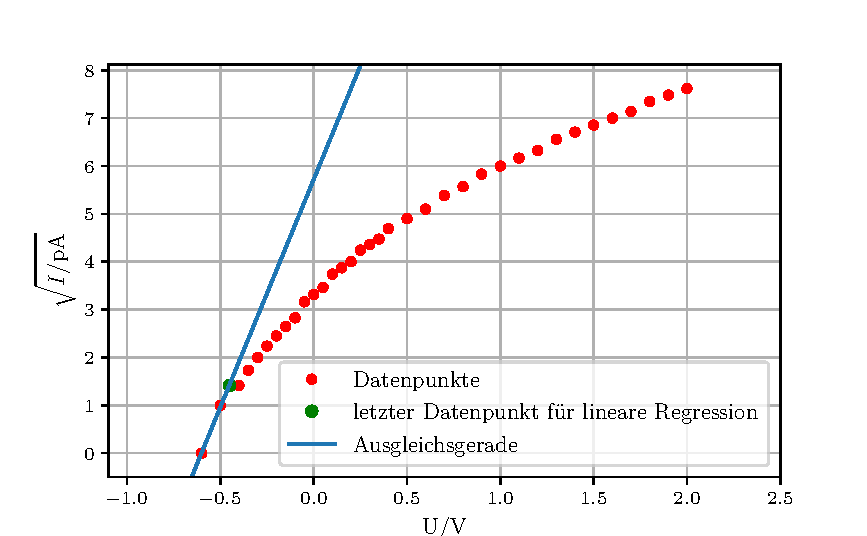
\includegraphics{content/rot.pdf}
  \caption{Messung der Stromabhängigkeit bei Variation der Brems-/Beschleunigungsspannung der roten Spektrallinie}
  \label{fig:rot}
\end{figure}
\begin{figure}[H]
  \centering
  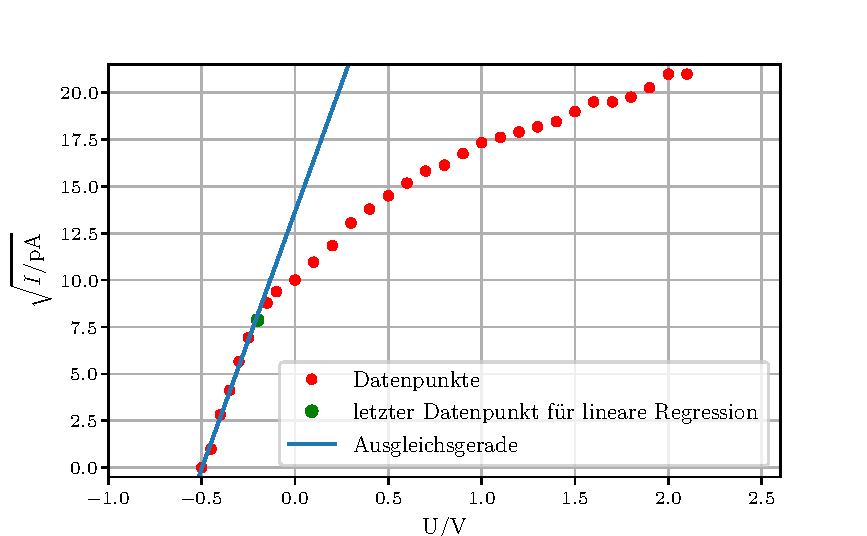
\includegraphics{content/gelb.pdf}
  \caption{Messung der Stromabhängigkeit bei Variation der Brems-/Beschleunigungsspannung der gelben Spektrallinie im Grenzbereich}
  \label{fig:gelb}
\end{figure}
\begin{figure}[H]
  \centering
  \includegraphics{content/grün.pdf}
  \caption{Messung der Stromabhängigkeit bei Variation der Brems-/Beschleunigungsspannung der grünen Spektrallinie}
  \label{fig:grün}
\end{figure}
\begin{figure}[H]
  \centering
  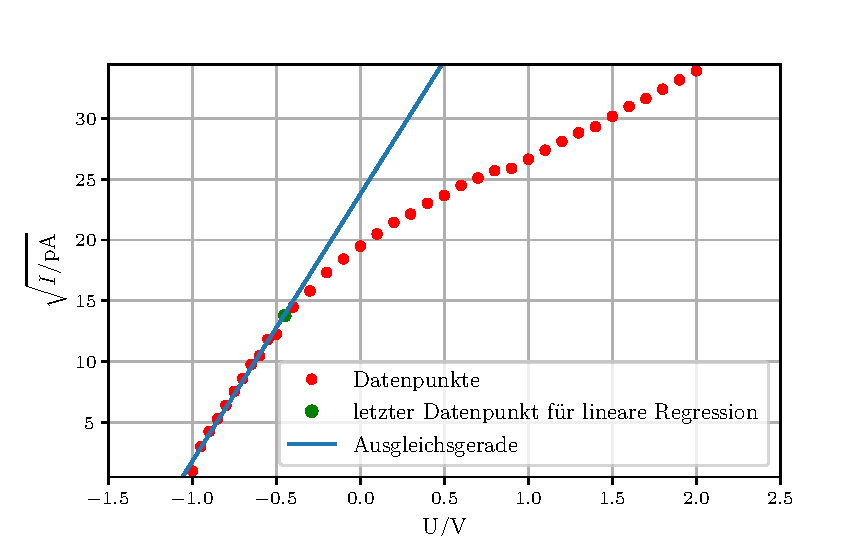
\includegraphics{content/lila.pdf}
  \caption{Messung der Stromabhängigkeit bei Variation der Brems-/Beschleunigungsspannung der violetten Spektrallinie}
  \label{fig:violett}
\end{figure}
\subsection{20V-Messung}
\begin{table}[H]
  \centering
  \caption{Messwerte für die gelbe Spektrallinie von -20V bis 20V.}
  \label{tab:20VMesswerte}
  \begin{tabular}{S[table-format=2.1] S[table-format=2] S[table-format=1.2] S[table-format=2]S[table-format=1.2]S[table-format=3]S[table-format=1.1]S[table-format=3]S[table-format=2.1]S[table-format=4]}
      \toprule
      {$U$/V}&{$I_\text{Ph}$/pA}&{$U$/V}&{$I_\text{Ph}$/pA}&{$U$/V}&{$I_\text{Ph}$/pA}&{$U$/V}&{$I_\text{Ph}$/pA}&{$U$/V}&{$I_\text{Ph}$/pA}\\
      \midrule
      -19 & -16 & -4 & -10 & -0,25 & 48 & 2,6 & 500 & 6,2 & 800 \\
      -18,5 & -16 & -3,5 & -10 & -0,2 & 62 & 2,7 & 520 & 6,4 & 800 \\
      -18 & -15 & -3 & -10 & -0,15 & 77 & 2,8 & 540 & 6,6 & 820 \\
      -17,5 & -15 & -2,5 & -10 & -0,1 & 88 & 2,9 & 560 & 6,8 & 820 \\
      -17 & -15 & -2,4 & -9 & 0 & 100 & 3 & 570 & 7 & 840 \\
      -16,5 & -14 & -2,3 & -9 & 0,1 & 120 & 3,1 & 580 & 7,2 & 860 \\
      -16 & -14 & -2,2 & -9 & 0,2 & 140 & 3,2 & 600 & 7,4 & 880 \\
      -15,5 & -14 & -2,1 & -9 & 0,3 & 170 & 3,3 & 620 & 7,6 & 880 \\
      -15 & -14 & -2 & -9 & 0,4 & 190 & 3,4 & 620 & 7,8 & 900 \\
      -14,5 & -14 & -1,9 & -9 & 0,5 & 210 & 3,5 & 640 & 8 & 920 \\
      -14 & -14 & -1,8 & -9 & 0,6 & 230 & 3,6 & 650 & 8,2 & 920 \\
      -13,5 & -14 & -1,7 & -9 & 0,7 & 250 & 3,7 & 660 & 8,4 & 920 \\
      -13 & -14 & -1,6 & -9 & 0,8 & 260 & 3,8 & 680 & 8,6 & 920 \\
      -12,5 & -14 & -1,5 & -9 & 0,9 & 280 & 3,9 & 670 & 8,8 & 920 \\
      -12 & -13 & -1,4 & -9 & 1 & 300 & 4 & 680 & 9 & 920 \\
      -11,5 & -13 & -1,3 & -8 & 1,1 & 310 & 4,1 & 680 & 9,5 & 940 \\
      -11 & -13 & -1,2 & -8 & 1,2 & 320 & 4,2 & 680 & 10 & 960 \\
      -10,5 & -13 & -1,1 & -8 & 1,3 & 330 & 4,3 & 680 & 10,5 & 980 \\
      -10 & -13 & -1 & -8 & 1,4 & 340 & 4,4 & 680 & 11 & 1000 \\
      -9,5 & -12 & -0,9 & -8 & 1,5 & 360 & 4,5 & 700 & 11,5 & 1000 \\
      -9 & -12 & -0,8 & -7 & 1,6 & 380 & 4,6 & 700 & 12 & 1000 \\
      -8,5 & -12 & -0,7 & -6 & 1,7 & 380 & 4,7 & 700 & 12,5 & 1000 \\
      -8 & -12 & -0,65 & -5 & 1,8 & 390 & 4,8 & 700 & 13 & 1000 \\
      -7,5 & -12 & -0,6 & -4 & 1,9 & 410 & 4,9 & 700 & 14 & 1000 \\
      -7 & -11 & -0,55 & -2 & 2 & 440 & 5 & 710 & 15 & 1000 \\
      -6,5 & -11 & -0,5 & 0 & 2,1 & 440 & 5,2 & 720 & 16 & 1000 \\
      -6 & -11 & -0,45 & 1 & 2,2 & 460 & 5,4 & 720 & 17 & 1100 \\
      -5,5 & -10 & -0,4 & 8 & 2,3 & 470 & 5,6 & 720 & 18 & 1100 \\
      -5 & -10 & -0,35 & 17 & 2,4 & 480 & 5,8 & 760 & 19 & 1100 \\
      -4,5 & -10 & -0,3 & 32 & 2,5 & 500 & 6 & 780 &  &  \\
      \bottomrule
  \end{tabular}
\end{table}

\begin{figure}[H]
  \centering
  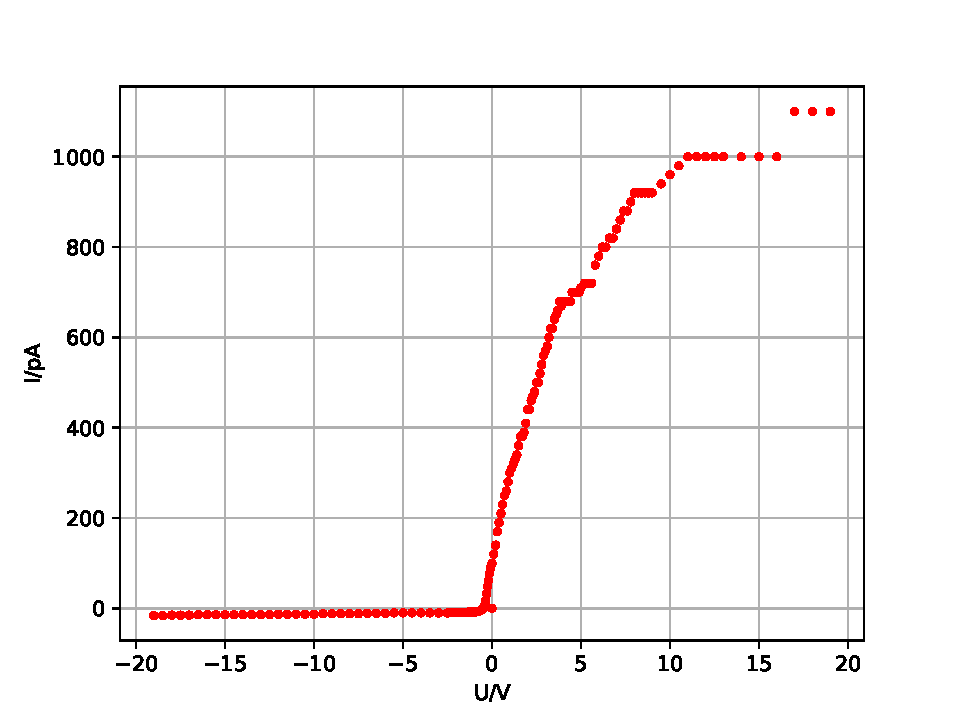
\includegraphics{content/Allgelb.pdf}
  \caption{Messung der Stromabhängigkeit bei Variation der Brems-/Beschleunigungsspannung der gelben Spektrallinie im gesamten 20V Bereich}
  \label{fig:rot}
\end{figure}
\subsection{Bestimmung der Grenzspannung und h/e$_0$}

\begin{figure}[H]
  \centering
  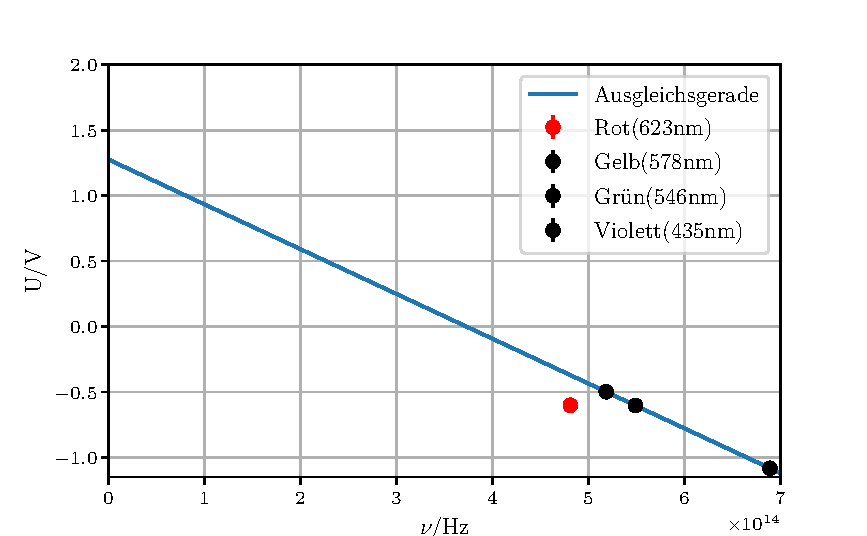
\includegraphics{content/Grenzspannung.pdf}
  \caption{Grenzspannungen der verschiedenen Spektrallinien}
  \label{fig:Grenz}
\end{figure}